\subsection{Optimización de refinería}
\subsubsection{Enunciado}
\paragraph{} Una refinería de aceite compra dos aceites crudos (crudo 1 y crudo 2). Estos aceites crudos se someten a cuatro procesos: destilación, reforma, craqueo y mezclado, para producir gasolinas y combustibles que se venden.
\paragraph{Distilación} La destilación separa cada aceite crudo en fracciones conocidas como nafta liviana, nafta media, nafta pesada, aceite liviano, aceite pesado y residuos según sus puntos de ebullición. Las naftas ligeras, medianas y pesadas tienen números de octano de 90, 80 y 70, respectivamente. Cada barril crudo produce: \\
\begin{center}
\begin{tabular}{ccccccc}
\hline 
 & Nafta & Nafta & Nafta & Aceite & Aceite & Residuos \\ 
 & liviana & media & pesada & liviano & pesado &  \\ 
\hline 
Crudo 1 & 0.1 & 0.2 & 0.2 & 0.12 & 0.2 & 0.13 \\ 
Crudo 2 & 0.15 & 0.25 & 0.18 & 0.08 & 0.19 & 0.12 \\ 
\hline 
\end{tabular} 
\end{center}
\paragraph{Reforma} Las naftas pueden usarse inmediatamente para mezclarse en diferentes grados de gasolina o pueden pasar por un proceso conocido como reforma. La reforma produce un producto conocido como gasolina reformada con un índice de octano de 115. Los rendimientos de gasolina reformada de cada barril de las diferentes naftas se dan de la siguiente manera:
\begin{itemize}
\item El barril de nafta liviana produce 0.6 barriles de gasolina reformada.
\item El barril de nafta mediana produce 0.52 barriles de gasolina reformada.
\item El barril de nafta pesada produce 0.45 barriles de gasolina reformada.
\end{itemize} 
\paragraph{Craqueo} 
Los aceites (livianos y pesados) se pueden usar directamente para mezclarlos en combustible para aviones o aceite combustible mediante un proceso conocido como craqueo catalítico. El craqueador catalítico produce aceite craqueado y gasolina craqueada. La gasolina craqueada tiene un octanaje de 105. 
\begin{itemize}
\item El barril de aceite liviano produce 0,68 barriles de aceite craqueado y 0,28 barriles de gasolina craqueada;
\item El barril de aceite pesado produce 0,75 barriles de aceite craqueado y 0,20 barriles de gasolina craqueada
\end{itemize} 
\paragraph{} El aceite craqueado se usa para mezclar aceite combustible y combustible para aviones; gasolina craqueada se utiliza para mezclar gasolina.
\paragraph{} Residuo se puede usar para producir aceite lubricante o mezclarlo en combustible para aviones y aceite combustible:
\begin{itemize}
\item El barril de residuos produce 0.5 barriles de aceite lubricante.
\end{itemize} 
\paragraph{Mezcla}
\begin{description}
\item[Gasolinas(combustible de motor)] Hay dos tipos de gasolina, regular y premium, obtenidos mezclando la nafta, la gasolina reformada y la gasolina crakeada. Las únicas restricciones que deben cumplir es que la gasolina regular debe tener un octanaje de al menos 84 y la premium al menos 94. Se supone que los números de octano se mezclan linealmente por volumen.
\item[Combustible para aviones] La restricción con respecto al combustible para aviones es que su presión de vapor no debe exceder 1 kg cm2. Las presiones de vapor para aceites ligeros, pesados, craquedos y residuos son 1.0, 0.6, 1.5 y 0.05 kg cm2, respectivamente. Se puede suponer nuevamente que las presiones de vapor se mezclan linealmente por volumen.
\item[Aceite combustible] Para producir aceite combustible, aceite craqueado, aceite liviano, aceite pesado y residuo se deben mezclar en una proporción de 10: 4: 3: 1.\\
Existen limitaciones de disponibilidad y capacidad en las cantidades y procesos utilizados de la siguiente manera:
\begin{enumerate}
\item La disponibilidad diaria de crudo 1 es de 20000 barriles.
\item La disponibilidad diaria de crudo 2 es de 30000 barriles.
\item Como máximo 45000 barriles de crudo se pueden destilar por día.
\item Como máximo se pueden reformar 10000 barriles de nafta por día.
\item Como máximo 8000 barriles de aceite pueden ser craqueados por día.
\item La producción diaria de aceite lubricante debe estar entre 500 y 1000 barriles.
\item La gasolina premium debe ser al menos el 40\% de la producción de la gasolina regular.
\end{enumerate}
Las contribuciones de ganancias de la venta de los productos finales son (en peniques por barril) de la siguiente manera:\\
\begin{center}
\begin{tabular}{cc}
\hline 
Gasolina premium & 700 \\ 
Gasolina regular & 600 \\ 
Combustible para aviones & 400 \\ 
Aceite combustible & 350 \\ 
Aceite lubricante & 150 \\ 
\hline 
\end{tabular} 
\end{center}
\end{description}
\paragraph{}¿Cómo deberían planificarse las operaciones de la refinería para maximizar el beneficio total?
\subsubsection{Modelo}

$\begin{array}{l}
C_{i}:\mbox{cantidad de barriles de crudo i}\\
D_{i}:\mbox{cantidad destilado de barriles de crudo i}\\
NL:\mbox{cantidad de nafta liviana obtenida en el proceso de destilacion}\\
NM:\mbox{cantidad de nafta mediana obtenida en el proceso de destilacion}\\
NP:\mbox{cantidad de nafta pesada obtenida en el proceso de destilacion}\\
NL_{t}:\mbox{cantidad de nafta liviana usada para mezclar gasolina en t}\\
NM_{t}:\mbox{cantidad de nafta mediana usada para mezclar gasolina en t}\\
NP_{t}:\mbox{cantidad de nafta pesada usada para mezclar gasolina en t}\\
NLR:\mbox{cantidad de nafta liviana que se puede refinar}\\
NMR:\mbox{cantidad de nafta mediana que se puede refinar}\\
NPR:\mbox{cantidad de nafta pesada que se puede refinar}\\
GR_{t}:\mbox{cantidad de gasolina reformada usada para mezclar gasolina en t}\\
AL:\mbox{cantidad de aceite liviano obtenida en el proceso de destilacion}\\
AP:\mbox{cantidad de aceite pesado obtenida en el proceso de destilacion}\\
AL_{s}:\mbox{cantidad de aceite liviano usado para mezclar en s}\\
AP_{s}:\mbox{cantidad de aceite pesado usado para mezclar en s}\\
ALC:\mbox{cantidad de aceite liviano que se puede craquear}\\
APC:\mbox{cantidad de aceite pesado que se puede craquear}\\
GC_{t}:\mbox{cantidad de gasolina crakeada usada para mezclar gasolina en t}\\
AC_{s}:\mbox{cantidad de aceite crakeado para mezclar en s}\\

R_{q}:\mbox{cantidad de residuo para mezclar en q}\\
GPrem:\mbox{cantidad gasolina premiun mezclada}\\
GRegu:\mbox{cantidad gasolina regular mezclada}\\
CAvion:\mbox{cantidad combustible de avion mezclado}\\
AComb:\mbox{cantidad aceite combustible mezclado}\\
ALu:\mbox{cantidad de aceite lubricante}\\
\mbox{donde} \;\;\;\;\;\; i=1,2 \;\;\;\;\;\; t=p,r  \;\;\;\;\;\; s=ca,ac \;\;\;\;\;\; q=ca,ac,al  
\end{array}$

$$ \mbox{max } 700 \mbox{ GPrem} + 600 \mbox{ GRegu} + 400 \mbox{ CAvion} + 350 \mbox{ AComb} + 150 \mbox{ ALu} $$
\\ \\
\\ \\ 
s.a\\
\begin{equation}
C_{1} \leq 20000 
\end{equation}
\begin{equation}
C_{2} \leq 30000 
\end{equation}
\begin{equation}
D_{1} \leq C_{1} 
\end{equation}
\begin{equation}
D_{2} \leq C_{2} 
\end{equation}
\begin{equation}
D_{1} + D_{2} \leq 45000 
\end{equation}
%como maximo se pueden reformar 1000 barriles de nafta por dia: nafta liviana: 0.1C_{1}+0.15C_{2}, nafta mediana  0.2C_{1}+0.25C_{2}, nafta pesada  0.2C_{1}+0.18C_{2}
\begin{equation}
NL = 0.1D_{1}+0.15D_{2} 
\end{equation}
\begin{equation}
NM = 0.2D_{1}+0.25D_{2} 
\end{equation}
\begin{equation}
NP = 0.2D_{1}+0.18D_{2} 
\end{equation}
\begin{equation}
NL_{p} + NL_{r} \leq NL 
\end{equation}
\begin{equation}
NM_{p} + NM_{r} \leq NM 
\end{equation}
\begin{equation}
NP_{p} + NP_{r} \leq NP 
\end{equation}
\begin{equation}
NLR = NL - (NL_{p} + NL_{r}) 
\end{equation}
\begin{equation}
NMR = NM - (NM_{p} + NM_{r}) 
\end{equation}
\begin{equation}
NPR = NP - (NP_{p} + NP_{r}) 
\end{equation}
\begin{equation}
GR_{p} + GR_{r} \leq 0.6 NLR + 0.52 NMR + 0.45 NPR 
\end{equation}
\begin{equation}
NLR + NMR + NPR \leq 10000 
\end{equation}
\begin{equation}
AL = 0.12D_{1}+0.08D_{2}
\end{equation}
\begin{equation}
AP = 0.19D_{1}+0.12D_{2}
\end{equation}
\begin{equation}
AL_{ca} + AL_{ac} \leq AL
\end{equation}
\begin{equation}
AP_{ca} + AP_{ac} \leq AP
\end{equation}
\begin{equation}
ALC = AL - (AL_{ca} + AL_{ac})
\end{equation}
\begin{equation}
APC = AP - (AP_{ca} + AP_{ac})
\end{equation}
\begin{equation}
ALC + APC \leq 8000 
\end{equation}
\begin{equation}
AC_{ca} + AC_{ac} \leq 0.68 ALC + 0.75 APC
\end{equation}
\begin{equation}
GC_{p} + GC_{r} \leq 0.28 ALC + 0.20 APC
\end{equation}
\begin{equation}
R_{ca} + R_{ac} + R_{al} \leq 0.13D_{1} + 0.12D_{2} 
\end{equation}
\begin{equation}
ALu \leq 0.5 R_{al} 
\end{equation}
\begin{equation}
ALu \geq 500 
\end{equation}
\begin{equation}
ALu \leq 1000 
\end{equation}
\begin{equation}
GPrem \leq NL_{p}+NM_{p}+NP_{p}+GR_{p}+GC_{p}
\end{equation}
\begin{equation}
GReg \leq NL_{r}+NM_{r}+NP_{r}+GR_{r}+GC_{r}
\end{equation}
\begin{equation}
(90NL_{p}+80NM_{p}+70NP_{p}+115GR_{p}+105GC_{p}) \div GPrem \geq 94 
\end{equation}
\begin{equation}
(90NL_{r}+80NM_{r}+70NP_{r}+115GR_{r}+105GC_{r}) \div GReg \geq 84 
\end{equation}
\begin{equation}
(GPrem \times 100) \div GReg \leq 40 
\end{equation}
\begin{equation}
CAvion \leq AL_{ca}+AP_{ca}+ AC_{ca}+ R_{ca}
\end{equation}
\begin{equation}
(1.0AL_{ca}+0.6AP_{ca}+1.5AC_{ca}+0.05R_{ca}) \div CAvion \leq 1 
\end{equation}
\begin{equation}
AComb \leq (1/10)AL_{ac}+(1/4)AP_{ac}+ (1/3)AC_{ac}+ R_{ac}
\end{equation}

\subsubsection{Modelo CPLEX}
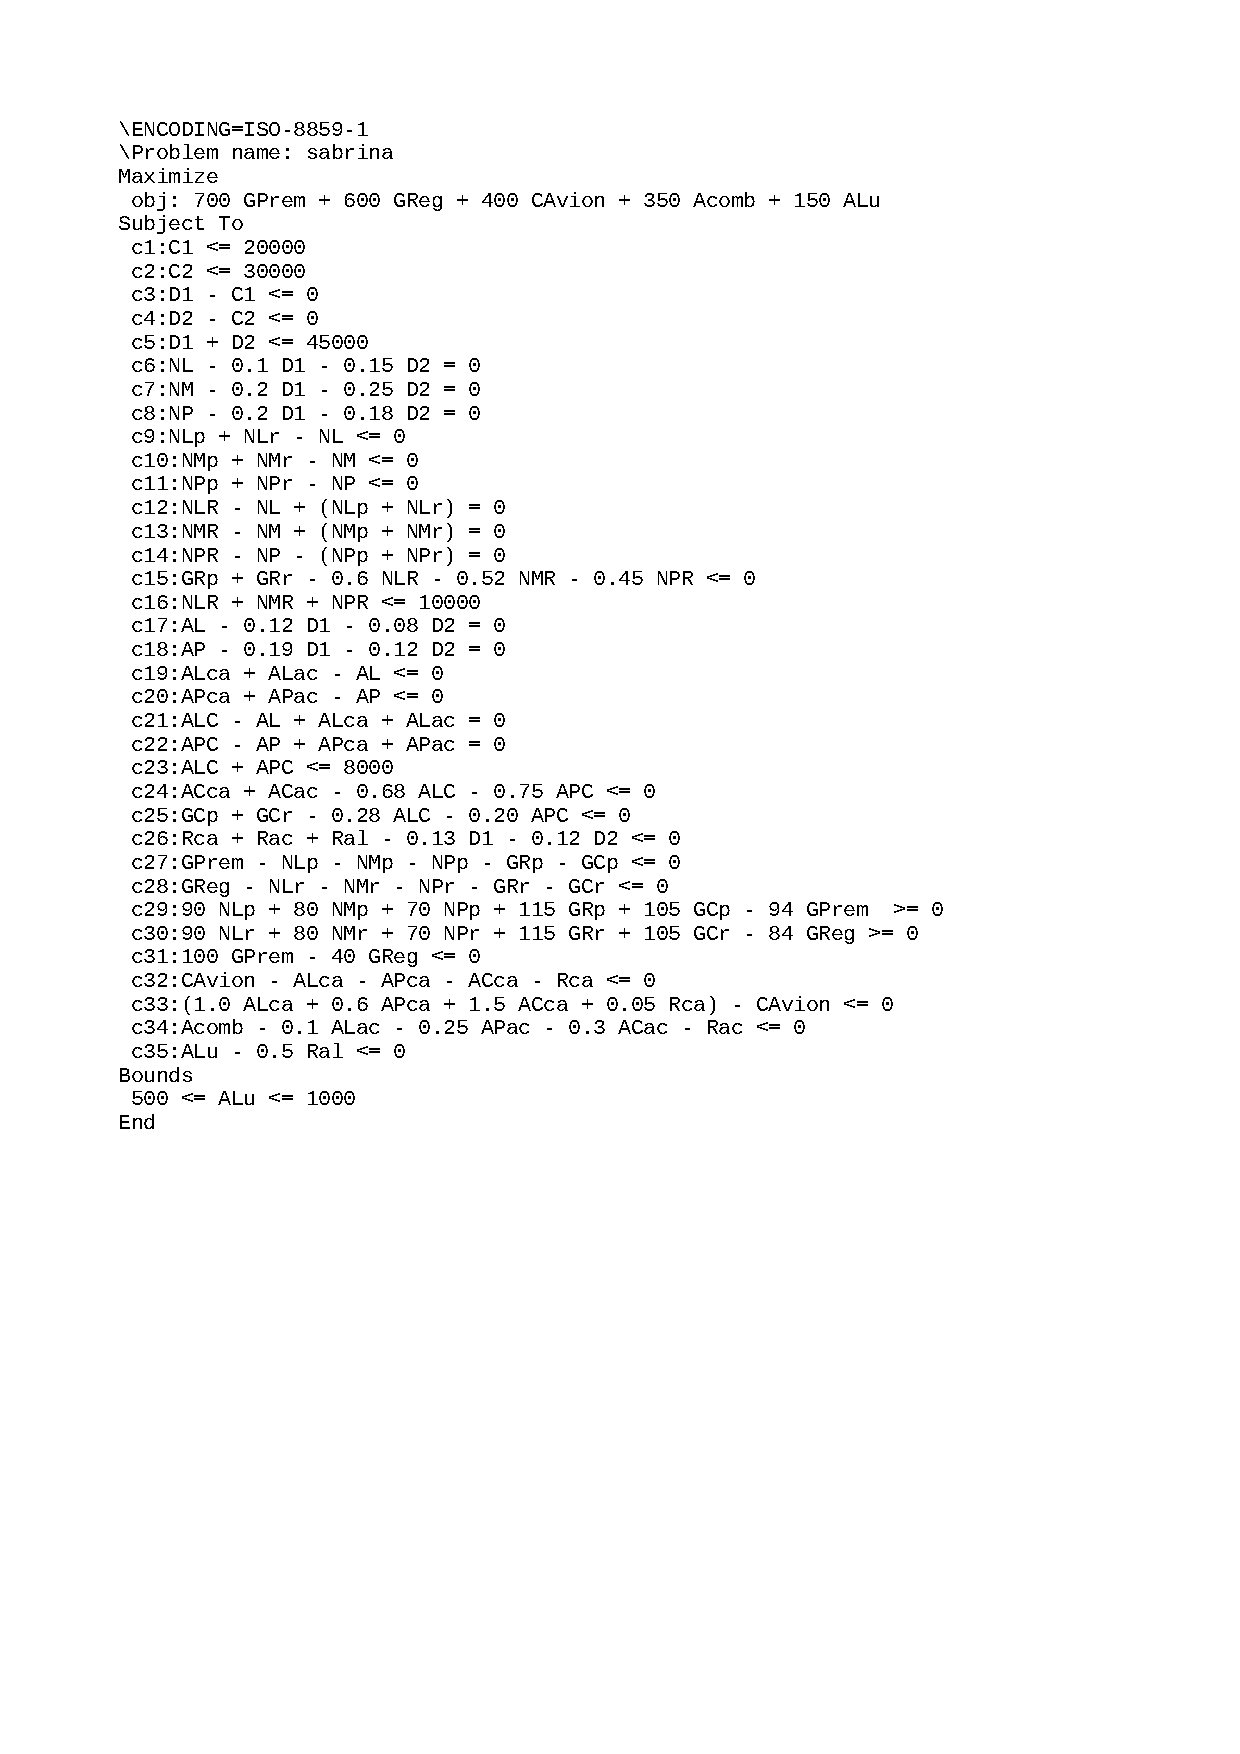
\includepdf[pages=1]{modelos/refineria}
\subsubsection{Solucion CPLEX}
\begin{figure}[!h]
    \centering
    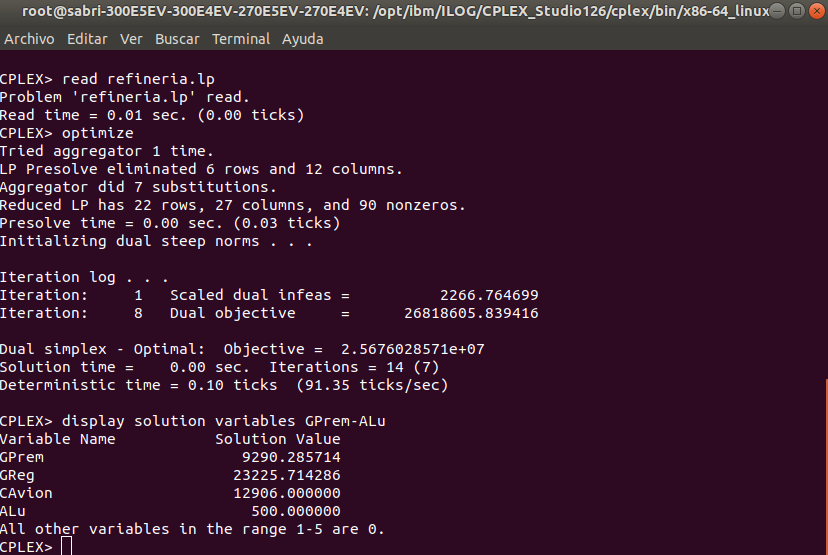
\includegraphics[scale=0.4]{modelos/SolutionRefineria.png}
    \caption{SolucionRefineria}
\end{figure}

